
\begin{frame}
  \frametitle{Big $\mathcal{O}$ notation}
\begin{itemize}
  \item <1-> Time complexity of an algorithm
  \item <2-> How many multiplications in a function
  \item <3-> Drop Constants
\end{itemize}
\end{frame}


\begin{frame}
  \frametitle{Big $\mathcal{O}$ notation}
  \onslide<1->{

  \begin{algorithm}[H]\caption{Square Matrix Multiplication}
    \setlength{\lineskip}{7pt}
    \begin{algorithmic}[1]
      \Function{foo}{$a, b$}
        \State \textbf{return} $a+b$
     \EndFunction
    \end{algorithmic}
  \end{algorithm}
}
\onslide<2->{
$\mathcal{O}(1)$
  }
\end{frame}

\begin{frame}
  \frametitle{Big $\mathcal{O}$ notation}
  \onslide<1->{

  \begin{algorithm}[H]\caption{Square Matrix Multiplication}
    \setlength{\lineskip}{7pt}
    \begin{algorithmic}[1]
      \Function{foo}{$a, b$}
        \State $ x \gets a+b $
        \State $ y \gets a \cdot b $
        \State \textbf{return} $x+y$
     \EndFunction
    \end{algorithmic}
  \end{algorithm}
}
\onslide<2->{
$\mathcal{O}(1) + \mathcal{O}(1) = 2\mathcal{O}(1) = \mathcal{O}(1) $
  }
\end{frame}

\begin{frame}
  \frametitle{Big $\mathcal{O}$ notation}
  \onslide<1->{

  \begin{algorithm}[H]\caption{Square Matrix Multiplication}
    \setlength{\lineskip}{7pt}
    \begin{algorithmic}[1]
      \Function{foo}{$\mathbf{A}, \mathbf{B}$,n}
      \State $ sum \gets 0$
      \For{$i = 0,1,2 \dots,n$}
        \State $ sum \gets sum + A[i] \cdot B[i] $
        \EndFor

        \State \textbf{return} $sum$

     \EndFunction
    \end{algorithmic}
  \end{algorithm}
}
\onslide<2->{
$\mathcal{O}(n)$
  }
\end{frame}

\begin{frame}
  \frametitle{Big $\mathcal{O}$ notation}
  \onslide<1->{

  \begin{algorithm}[H]\caption{Square Matrix Multiplication}
    \setlength{\lineskip}{7pt}
    \begin{algorithmic}[1]
      \Function{foo}{$\mathbf{A}, \mathbf{B}$,n}
      \State $ sum \gets 0$
      \For{$i = 0,1,2 \dots,n$}
      \For{$j = 0,1,2 \dots,n$}
      \State $ sum \gets sum + A[i] \cdot B[j] $
      \EndFor
      \EndFor
        \State \textbf{return} $sum$
     \EndFunction
    \end{algorithmic}
  \end{algorithm}
}
\onslide<2->{
$\mathcal{O}(n^2)$
  }
\end{frame}


\begin{frame}
  \frametitle{Big $\mathcal{O}$ notation}
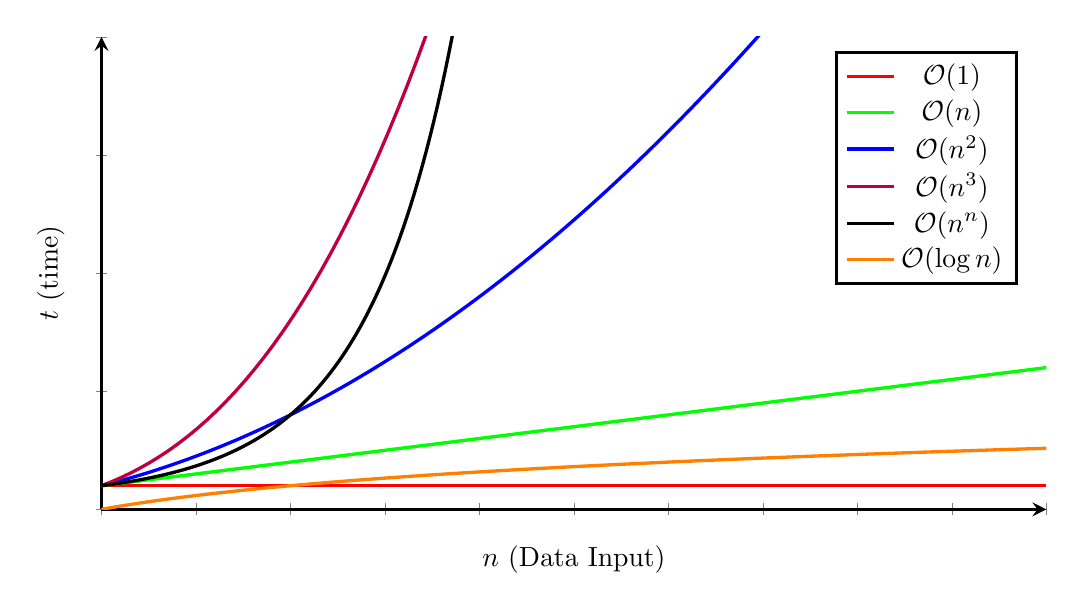
\begin{tikzpicture}
\begin{axis}[
    axis lines = left,
    xlabel = $n$ (Data Input),
    ylabel = {$t$ (time)},
    legend pos=north east,
    very thick,
    ymax = 20,
    yticklabels=\empty,
    xticklabels=\empty,
    scale only axis=true,
  width=12cm, height=6cm,
    ]
%Below the red parabola is defined
\addplot [
    domain= 1:6,
    samples=100,
    color=red,
]
{1};
\addlegendentry{$\mathcal{O}(1)$}
%Here the blue parabloa is defined
\addplot [
    domain= 1:6,
    samples=100,
    color=green,
]
{x};
\addlegendentry{$\mathcal{O}(n)$}
\addplot [
    domain= 1:6,
    samples=100,
    color=blue,
]
{x^2};
\addlegendentry{$\mathcal{O}(n^2)$}
\addplot [
    domain= 1:6,
    samples=100,
    color=purple,
]
{x^3};
\addlegendentry{$\mathcal{O}(n^3)$}
\addplot [
    domain= 1:3,
    samples=100,
    color=black,
]
{x^x};
\addlegendentry{$\mathcal{O}(n^n)$}
\addplot [
    domain= 1:6,
    samples=100,
    color=orange,
]
{log2(x)};
\addlegendentry{$\mathcal{O}(\log n)$}
\end{axis}
\end{tikzpicture}

\end{frame}
